\documentclass[tikz, border=2pt]{standalone}

\usepackage{helvet}
\renewcommand{\familydefault}{\sfdefault}

\usepackage[EULERGREEK]{sansmath}
\sansmath
\usetikzlibrary{arrows.meta}

\begin{document}%

\begin{tikzpicture}[line width=2pt]
\tikzset{>={Latex[width=3mm,length=4mm]}}

% grid
%\draw[help lines] (-0.5, 3) grid (10, 15);



  \node[inner sep=0pt] (figa) at (4.5,12.8)
  {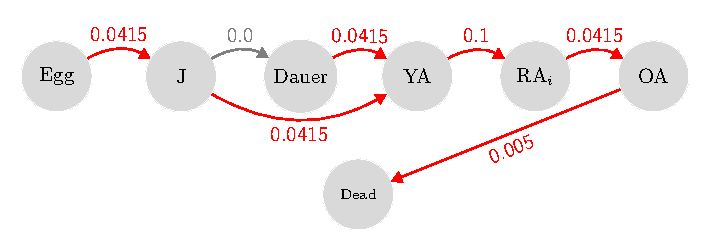
\includegraphics[width=0.75\textwidth]{./tikz_figs/markov_chain_R_OP50.pdf}};

  \node[inner sep=0pt] (figa) at (4.5,9.)
  {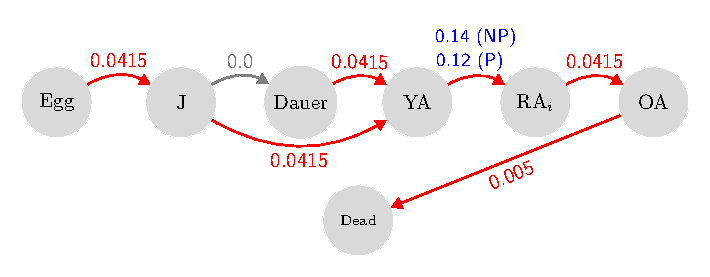
\includegraphics[width=0.75\textwidth]{./tikz_figs/markov_chain_R_Novo.pdf}};

  \node[inner sep=0pt] (figa) at (4.5,5.)
  {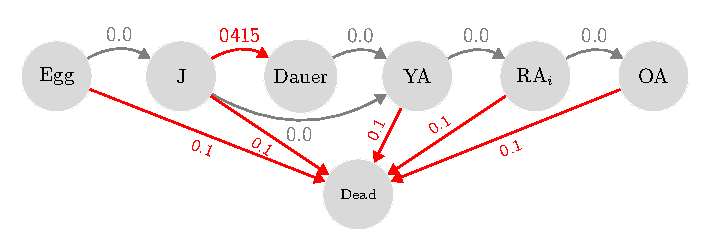
\includegraphics[width=0.75\textwidth]{./tikz_figs/markov_chain_NR.pdf}};



\node at (4.3,14.7) [draw=none, rectangle, rotate=0] (g1) {\sf \large \emph{E. coli} OP50};

\node at (4.3,10.7) [draw=none, rectangle, rotate=0] (g1) {\sf \large \emph{Novosphingobium} sp. L76};

\node at (4.3,6.8) [draw=none, rectangle, rotate=0] (g1) {\sf \large Low resource};


%labels
\draw (0., 15) node{{\Huge\sf\textbf{a}}};

\draw (0., 11.) node{{\Huge\sf\textbf{b}}};

\draw (0., 7) node{{\Huge\sf\textbf{c}}};

\end{tikzpicture}


\end{document}